\chapter{Execution}\label{sec:Execution}
To start a Varroa test the user needs to start a Commander and at least one Agent.
The Agents periodically tries to establish a connection to the Commander.
Once all Agents are connected the execution of the scenario starts.\\

\section{Commander}
\begin{figure}[H]
	\begin{center}
	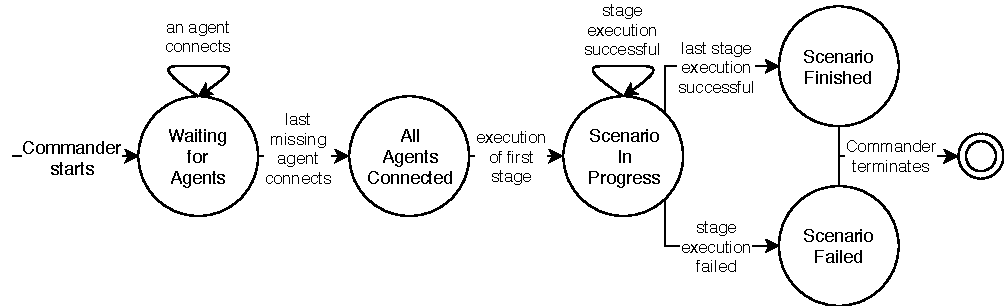
\includegraphics[scale=0.9]{Resources/PDF/CommanderStates}
	\caption{Commander States}
	\label{pic:CommanderStates}
	\end{center}
\end{figure}
When starting a Varroa Instance that is configured as a Commander (see \ref{sec:commanderConfig}) it performs the following actions:
\begin{itemize}
	\item First it parses and validates the Scenario.
	\item Then it waits for the Agents to connect.
	Until all Agents are successfully connected it remains in the \emph{Waiting for Agents} state.
	As the last missing Agent has connected to the Commander it switches its state to \emph{All Agents Connected}.
	\item When all Agents are connected, the Commander starts to distribute the Scenario data amongst the Agents. After this is finished the state is set to \emph{Scenario Data Distributed}.
	\item After the preceding initiation steps the actual distribution and execution of the Scenario is started.
	In doing so the Commander changes its state to \emph{Scenario in Progress}.
	In this state it distributes the Stages of the Scenario one after each other to the Agents.
	It remains in this state until all Stages are successfully executed and then transfers its state into \emph{Scenario Finished}.
	If one execution of a Stage errors this results in the failure of the whole Scenario -- logically the Commanders state is then \emph{Scenario Failed}.
	\item As the last step the Commander always -- independent of execution success -- generates the final Report by aggregating the partial reports from the Agents.
\end{itemize}

To allow better comprehension \figurename{} \ref{pic:CommanderStates} illustrates this process.

\section{Agent}
\begin{figure}[H]
	\begin{center}
	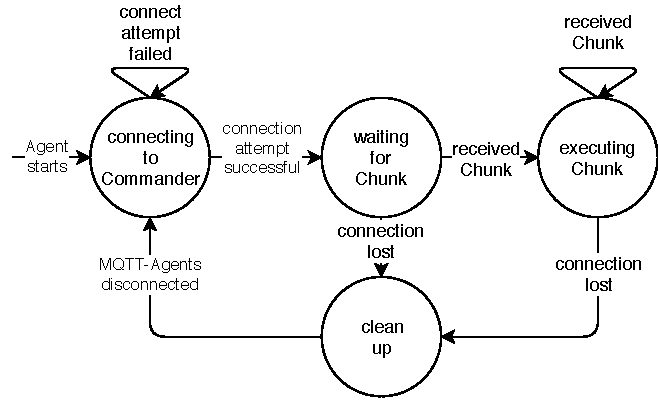
\includegraphics[scale=0.9]{Resources/PDF/AgentStates}
	\caption{Agent States}
	\label{pic:AgentStates}
	\end{center}
\end{figure}
Upon starting a Varroa Instance as an Agent (see \ref{sec:agentConfig}) it performs the following actions:
\begin{itemize}
	\item First it tries to connect to the configured Commander.
	It periodically attempts to establish the connection until it succeeds.
	\item Then it waits for incoming Chunks from the Commander and executes them, implementing the handshake protocol that will be introduced in \ref{sec:chunkDistribution}.
	The Agent continues doing so until the Connection is closed by the Commander, which means the Scenario is executed completely.
	\item In contrast to the Commander the Agent process does not terminate after the execution of a Scenario. Instead it returns to the first step and tries to reconnect to a Commander.
	Because of this the user only needs to restart the Commander to execute another Scenario.
\end{itemize}

For better understanding of the temporal processes the just explained concepts are illustrated in figure \ref{pic:AgentStates}.

\section{Configuration}
Varroa can be run with two different ways of configuration.
One is to configure Varroa ahead of time -- manually or programmatically.
The other is to use containers and utilize dynamic discovery of the Varroa Instances.

\subsection{Static configuration}
\begin{figure}[h]
\begin{center}
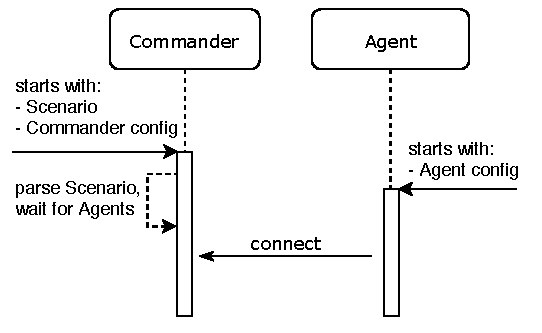
\includegraphics[scale=1]{Resources/PDF/ExecutionStaticInit}
\caption{Static configuration}
\label{pic:staticExecution}
\end{center}
\end{figure}

A static configuration may be used on any infrastructure where the hostnames or IP addresses of all Varroa Instances (Commander and Agents) are known ahead of time. This is the case on most of the typically used systems, such as IaaS clouds where an instance is booted and is assigned an address before the application is deployed onto the system.\\
\\
To configure Varroa statically the user must provide an Instance configuration, which sets up the Varroa Instance as a Commander or an Agent.
It is also possible to configure a single Varroa Instance as both Commander and Agent.
This allows simple execution of small tests on a single machine.
\\
If the Varroa Instance is configured as a Commander the user must also provide a Scenario.
\\
Both Instance configuration and the Scenario are defined in XML files.
These are referenced by the command line parameters -I and -S:
\begin{lstlisting}[caption={Command line configuration examples}, captionpos=b, label={lst:commanderConfig}, language=bash]
java -jar varroa-1.0.jar -I path/to/commander.xml -S path/to/scenario.xml
java -jar varroa-1.0.jar -I path/to/agent.xml
\end{lstlisting}

A detailed description of the Instance configuration options can be found below.

\subsubsection{Commander configuration}\label{sec:commanderConfig}
\begin{lstlisting}[caption={Commander XML configuration example}, captionpos=b, label={lst:commanderConfig}, language=XML]
<varroa>
    <commander>
		<bind-host>192.127.0.1</bind-host>
        <bind-port>12345</bind-port>
        <amount-agents>3</amount-agents>
    </commander>
</varroa>
\end{lstlisting}
\begin{itemize}
	\item \textbf{bind-host:} specifies the address the Commander will accept Agent connections on.
	\item \textbf{bind-port:} specifies the port the Commander waits for Agent connections on.
	\item \textbf{amount-agents:} specifies the amount of Agents that the Commander awaits.
\end{itemize}

\subsubsection{Agent configuration}\label{sec:agentConfig}
\begin{lstlisting}[caption={Agent XML configuration example}, captionpos=b, label={lst:agentConfig}, language=XML]
<varroa>
    <agent>
		<commander-host>192.127.0.1</commander-host>
        <commander-port>12345</commander-port>
        <local-port>23458</local-port>
		<commander-retry-interval>10</commander-retry-interval>
    </agent>
</varroa>
\end{lstlisting}
\begin{itemize}
	\item \textbf{commander-host:} specifies the address of the Commander to connect to.
	\item \textbf{commander-port:} specifies the port of the Commander.
	\item \textbf{local-port:} specifies the local port the Agent uses for the outgoing connection to the Commander.
	\item \textbf{commander-retry-interval:} the time interval in seconds in which the Agent tries to connect to the Commander.
\end{itemize}

\subsection{Dynamic configuration}

\begin{figure}[h]
\begin{center}
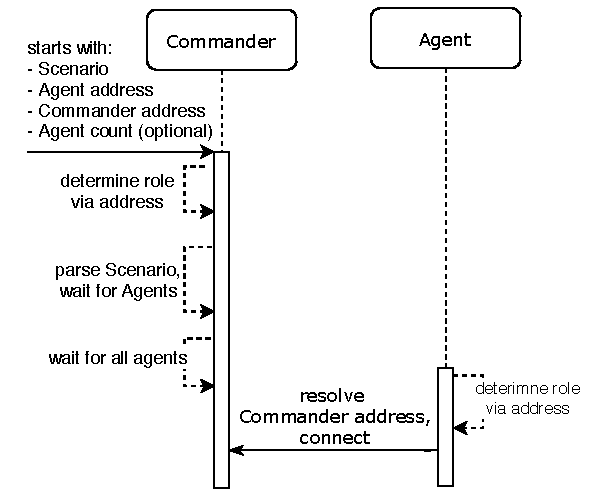
\includegraphics[scale=1]{Resources/PDF/ExecutionDnsInit}
\caption{dynamic execution}
\label{pic:dynamicExecution}
\end{center}
\end{figure}

DNS discovery is specifically aimed at container environments and cloud platforms. These types of platforms generally provide different methods of service discovery, which are necessary to allow the parts of a distributed system to communicate with each other.

In container environments, the address of a server where an application is going to run on is generally not known ahead of application startup. Containers are launched quickly and in an unpredictable order, leading to a scenario where the addresses of all parts of a system are unknown ahead of time. This necessitates a configuration method which allows service discovery after application startup, which the previous method cannot handle.


Dynamic configuration allows Varroa to start without knowing the addresses of any other Varroa instances nor its own role. The way the initial DNS discovery method works is by supplying hostnames for the Commander and Agent groups respectively.


\begin{figure}[h]
\begin{center}
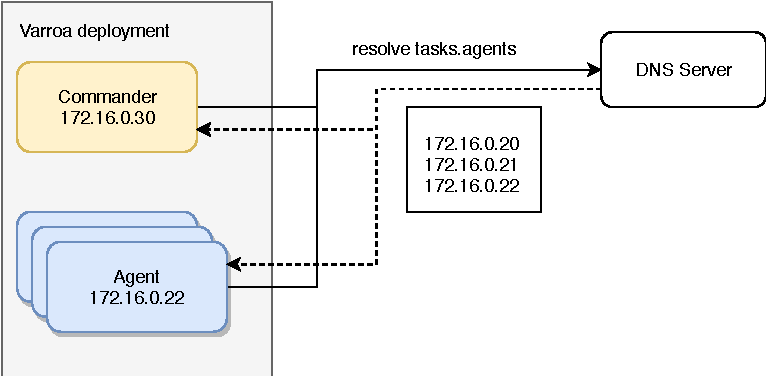
\includegraphics[scale=0.8]{Resources/PDF/ExecutionDnsDiscovery}
\caption{agent record resolution}
\end{center}
\end{figure}

During start up Varroa will continuously resolve these records, which must be designed as round-robins.
Then each address found in the records is compared to the address corresponding to its own hostname. 
If a match is found, the instance will set its role according to the set of addresses it matches.

Additionally, Agents can use the commander address to locate the commander node and continuously attempt to connect to it until it is ready for Agent connections.

The commander can also determine how many Agents will connect to it using the Agent address, or alternatively a Agent count can be  provided at startup (for deployments on services where records are slowly updated as containers start).

\begin{figure}[h]
\begin{lstlisting}
VARROA_DNS_AGENT=tasks.agents
VARROA_DNS_COMMANDER=tasks.commander
VARROA_DNS_AGENT_COUNT=3
\end{lstlisting}
\caption{A sample dynamic discovery configuration, showing the environment variable values}
\end{figure}
